\chapter{Event Reconstruction}
\label{chap:eventreco}

\section{Basic Elements From the Detector} 

Depending on their nature, the particles emanating from the collision leave various forms of energy deposits in the different subdetectors. All these signals need to be aggregated and processed to allow for the reconstruction of what could be considered particle-level information. The first step in this process consists of building \textit{Particle Flow elements} using information within each subdetector. There are four primary elements from the subdetectors: tracks from the tracker, calorimeter deposits in each of the ECAL and HCAL, and tracks from the muon detector. The elements are eventually combined via the \textit{Particle Flow algorithm}, yielding reconstructed particles used for physics analysis.

Note that the definition of any object within the detector makes use of additional selection criteria which are not generally discussed here. For instance, one may require that a track in the tracker have at least 3 hits in the pixel detector, or that a calorimeter hit is above some minimum threshold energy. The effects of these criteria are generally a balance between the reconstruction efficiency of any given particle and the probability to misidentify a particle (purity).

\subsection{Tracks}% \& Vertices}

Tracker hits are formed in the pixel and strips detectors by clustering any hits in neighboring elements of the detector plane. The cluster position is a weighted average of the individual channel positions. Charge sharing among detector channels allow for a finer spatial resolution in the position measurement. Track reconstruction first begins by forming track seeds consisting of a small number of detector hits. These track seeds are then projected onto successive detector layers looking for additional hits. This follows the Kalman filtering procedure, in which track information is updated after the addition of each hit \cite{trackerreco}.
 
The track building procedure follows an iterative procedure, where the requirements on the quality of the track seed decrease as the iterations proceed. After a given iteration the hits used in building the tracks are removed from subsequent iterations. The first iterations begin with seeds consisting of 3 pixel hits and lead to high performance reconstruction of high $p_{T}$ tracks emanating from the collision region. The iterations proceed until essentially only requiring hits in the outer tracker to reconstruct displaced tracks or tracks with missing hits. The iteration procedure provides a balance between reconstruction efficiency, purity, and computation economics. Table~\ref{tab:itertracks} lists these iterations; the requirements on the seeds and the type of tracks which are targeted.

\begin{table}[hbp!]
\caption
[Seeding requirements for each step in the iterative track reconstruction.]
{Seeding requirements for each step in the iterative track reconstruction \cite{CMS-PRF-14-001}.}
\centering
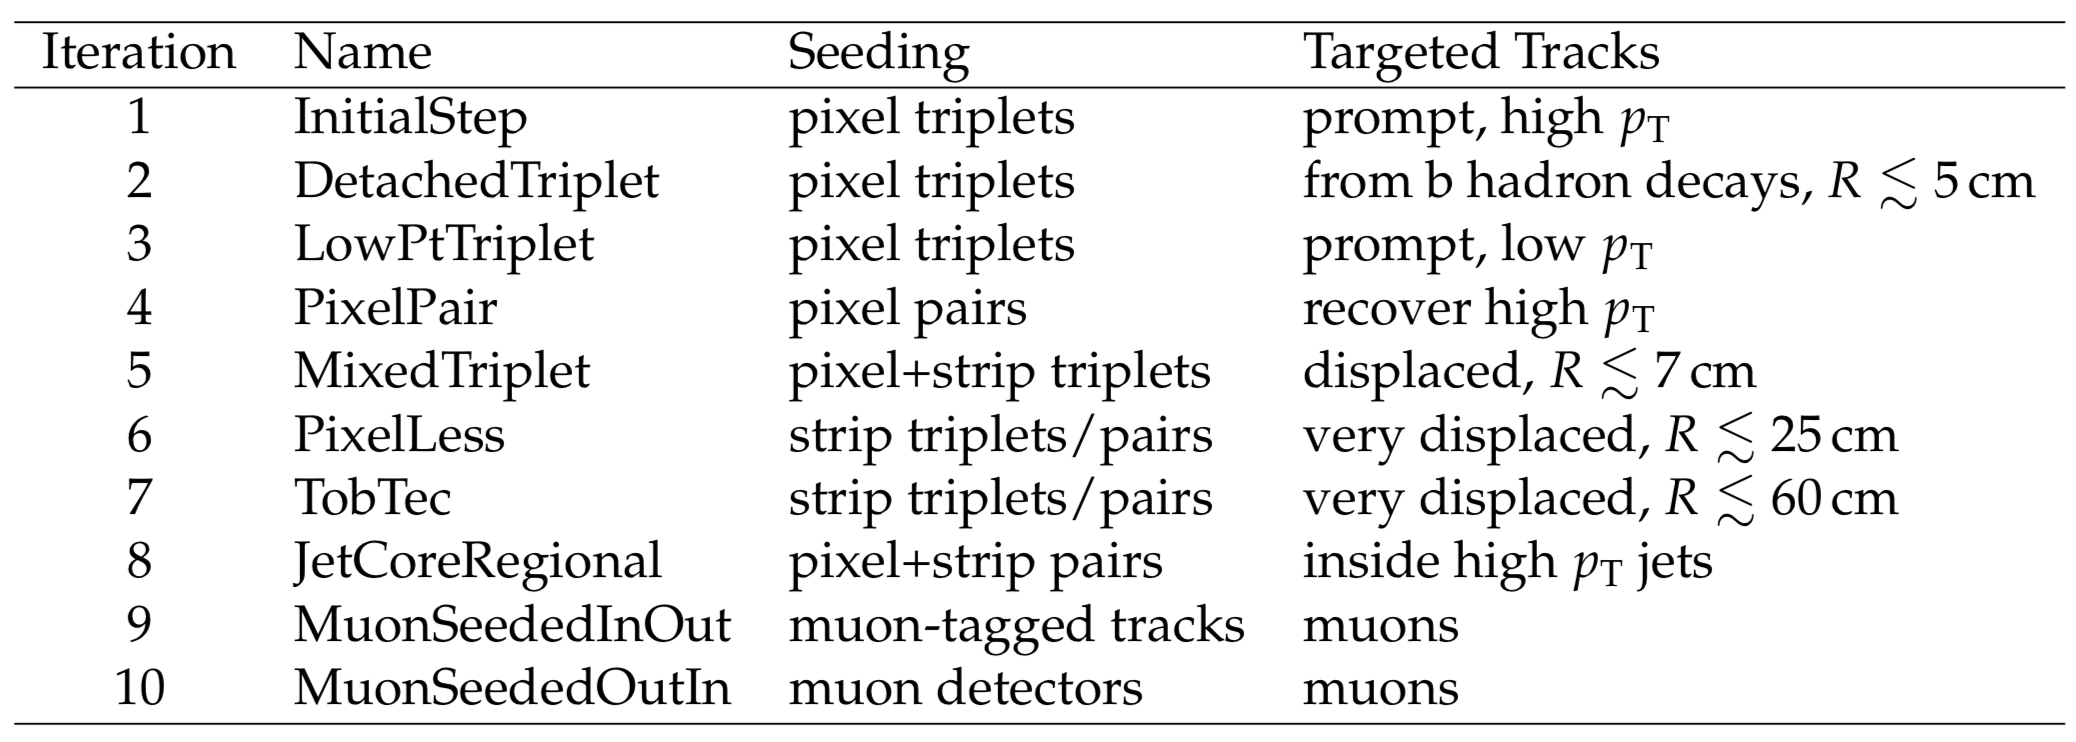
\includegraphics[width=0.8\textwidth]{figs/itertracks.png}
\label{tab:itertracks}
\end{table}

Electron tracking is performed with a modified Gaussian sum filter to account for the electron's energy loss in the detector. Electrons are very light and susceptible to emitting \textit{bremsstrahlung} radiation, occuring when the electron scatters from nucleus within the tracker and emits a photon. This results in non-neglible energy loss and changes in direction as the electron traverses the detector. This results in very non-Gaussian energy loss mechanisms in which the Kalman filtering is non-optimal.

\subsection{ECAL \& HCAL Clusters}

\textit{Superclusters} in the ECAL are built by first identifying a crystal with the largest energy deposit, this is called a \textit{seed}. The supercluster is then formed by aggregating any hits among the neighbors (up to 8) of the hits already in the cluster. This process then proceeds building all the superclusters and consuming all the calorimeter hits. Superclusters are built separately in the barrel and endcap. Within a given supercluster, N clusters are identified using an iterative algorithm assuming the observed hits arise from N Gaussian-distributed energy deposits; each of energy E, position in the $\eta-\phi$ plane $\vec{\mu}$, and width $\sigma$ scale set by the crystal size.

\subsection{Muon Tracks}

As there are multiple detector layers within a single muon station, track segments are locally formed within a chamber for both the DTs and CSC. These track segments represent the muon momentum at that station; pattern recognition is able to provide to measurement and its high speed allows the segments to be used trigger primitives for the muon systems. For track reconstruction, the track segments act as seeds for the track finding algorithm. The hits in each the DT, CSC, and RPC subdetectors are used in the final track reconstruction.

\section{Obtaining a Particle-level Description}

Once the elements have been built, the Particle Flow algorithm exploits the information from each of the detectors to form the best possible particle candidate \cite{CMS-PRF-14-001}. As different varieties of particles have unique signatures in the detector, particle identification is aided by the particular combination of elements \textit{linked} with one another. An illustrative example of these combinations are shown in Figure~\ref{fig:schematicview}.  Elements are linked when projections from one element to the other are spatially consistent. There are six primary links:

\begin{itemize}
\item Tracks formed in the tracker are linked to an ECAL or HCAL cluster if the projection of the track, at a depth of the expected maximum of a shower in the ECAL or at one interaction length inside the HCAL, lies within the cluster area.
\item ECAL and HCAL clusters are linked if the ECAL cluster falls within the envelope of the HCAL cluster; ECAL provides finer spatial resolution compared to the HCAL.
\item If a Preshower cluster is within the envelope of an ECAL cluster the two are linked; Preshower has finer spatial granularity.
\item A tracker track and a muon track are linked if their projections onto a common surface are spatially consistent.
\item To collect bremsstrahlung radiation (photons) associated to an electron track, an ECAL cluster is linked to tracker tracks if projections tangent to the track at any of the tracker layers lies within the cluster volume. To catch these bremsstrahlung photons which additionally then convert into an $e^{+}e^{-}$ pair in the tracker, track pairs consistent with $e^{+}e^{-}$ conversion as linked if their common momentum points to one of the track tangents.
\item Tracks consistent with arising from a secondary vertex are linked to allow for reconstruction of nuclear-interactions.
\end{itemize}

Particle Flow \textit{blocks} are constructed by aggregating objects directly or indirectly linked with one another. The Particle Flow algorithm then processes each block in turn to create the final reconstructed particles. The algorithm builds the objects in the following order

\begin{enumerate}
\item \textbf{Muons}:
There are three types of tracks which can be used for muon reconstruction:
\begin{itemize}
\item
\textit{\textbf{standalone}} muons are built from tracks reconstructed solely in the muon system.
\item
\textit{\textbf{tracker}} muons are built from tracks reconstructed solely in the inner silicon tracker. They are tagged as such if the track projection is consistent with any track segments found in the muon system.
\item
\textit{\textbf{global}} muons are reconstructed using the hits from both the inner silicon tracker and the muon stations. Global muons are reconstructed when a track in the tracker and a track in the muon system are compatible.
\end{itemize}

Any ECAL or HCAL clusters associated with the muon track are used as muon selection/definition criteria if those clusters are found to be consistent with the muon hypothesis.

\item \textbf{Electrons \& Photons}:

An electron is formed by combining a track in the silicon tracker with a cluster in the ECAL. Its energy assignment uses a combination of both elements. The momentum direction is made using the track in the silicon tracker, as it gives greater spatial resolution.  A photon is defined as an ECAL cluster not associated with a track. Surrounding energy in the HCAL must not exceed 10\% of the ECAL supercluster energy.

Electrons and isolated photons are reconstructed within the same Particle Flow step to account for similar behavior within the tracker bulk. There is a large probability for both a) an electron to radiate a brehmsstrahlung photon and b) for a photon to convert to an e$^{+}$e$^{-}$ pair. Therefore in object reconstruction care must be taken to collect the photons radiated from electrons in order to make appropriate measurements of the particles.

\item \textbf{Hadrons \& Photons}:

Hadrons \& non-isolated photons result from hadronization/fragmentation of jets. ECAL clusters not associated to any tracks are assigned to be photons. Neutral hadrons ($K^{0}_{L}$, neutrons) are reconstructed from HCAL clusters with no associated track; neutral hadrons leave a very small amount of energy in the ECAL. Charged hadrons ($\pi^{\pm}$, K$^{\pm}$, protons) are reconstructed using the remaining tracks and HCAL deposits.

\item \textbf{Nuclear Interactions}:

A nuclear interaction may occur when a hadron from the pp collision interacts with the detector material causing a shower of (charged and neutral) secondary particles. The tracks from the shower may be linked through a common (displaced) secondary vertex, in this case they will be replaced by a single charged hadron under the assumption of the pion mass.

\end{enumerate}

\section{Additional High-Level Objects}

\subsection{Jets}

Bare quarks and gluons can never be observed in Nature due to a QCD phenomenon called \textit{color confinement}. Therefore, quark and gluon production manifests as a ``jet'' of color-neutral particles emanating from the production point. These particles can be clustered together to reconstruct the original parton. The jets used in this analysis are made by clustering particles with the ``anti-kt`` algorithm with cone sizes of $\Delta R$ = 0.4, 0.8 \cite{1126-6708-2008-04-063}, denoted as AK4 and AK8 jets respectively. This algorithm produces nearly conical jets and is infrared and collinear safe. The AK4 jets subtend less solid angle and are used to capture the hadronisation of single quarks and gluons. AK8 jets subtend a larger solid angle and are used for reconstruction of boosted objects that decay to multiple jets.

\subsection{b-tagging of Jets}

Jets resulting from the production of b quarks (and to some extent c quarks) garner special attention in our experiment. As usual for quarks and gluons, the b-quark will quickly hadronize and form a b hadron. However, the lifetimes of b hadrons are such that it will generally travel hundreds of microns before decaying. Vertexing the tracks resulting from the decay will reveal the presence of a \textit{secondary vertex} which is spatially displaced from the primary vertex from which the other hadrons inside the jet originate. This secondary vertex allows for one handle on being able to identify jets as coming from b quark production. Other handles include the momenta and multiplicity of the other particles clustered into the jet.

In addition to tagging jets as originating from a single b quark, tagging of jets as originating from \textbf{two} b quarks is also possible \cite{bbtagger}.

\subsection{Invisible Particles $\rightarrow p_{T}^{\mathrm{miss}}$}

Neutrinos are so weakly interacting that they leave no energy deposits in CMS and are not detected by our experiment. Although direct detection is not possible, we are able to infer their presence. The net momentum of the protons involved in the collisions are zero, but the individual partons (quarks and gluons) within the proton carry unknown fractions of this total (longitudinal) momentum. Only in the transverse direction may we require momentum conservation. We define this imbalance as:

\begin{equation}
p_{T}^{\mathrm{miss}}  \equiv \left | - \sum_{i} \vec{p_{T}} \right |,~\forall~\textrm{particles~i}.
\end{equation}

If all particles in the event are perfectly reconstructed, $p_{T}^{\mathrm{miss}}$ would equal zero. Large values indicate the presence of an undetected particle, such as a SM neutrino or something more exotic like the light supersymmetric neutralinos $\chi^{0}_{0}, \chi^{0}_{1}$. This quantity is sometimes labeled as \textit{MET}.